\documentclass{article}

\usepackage{graphicx}
\usepackage{float}
\usepackage{amssymb}

\title{Machine Intelligence 2 - Exercise 9\\
Stochastic Optimization}
\author{Jens Krenzin - 319308\\
Till Rohrmann - 343756}
\date{\today}

\begin{document}
	\maketitle
	\setcounter{section}{9}
	\subsection{Simulated Annealing}
		\begin{figure}[H]
			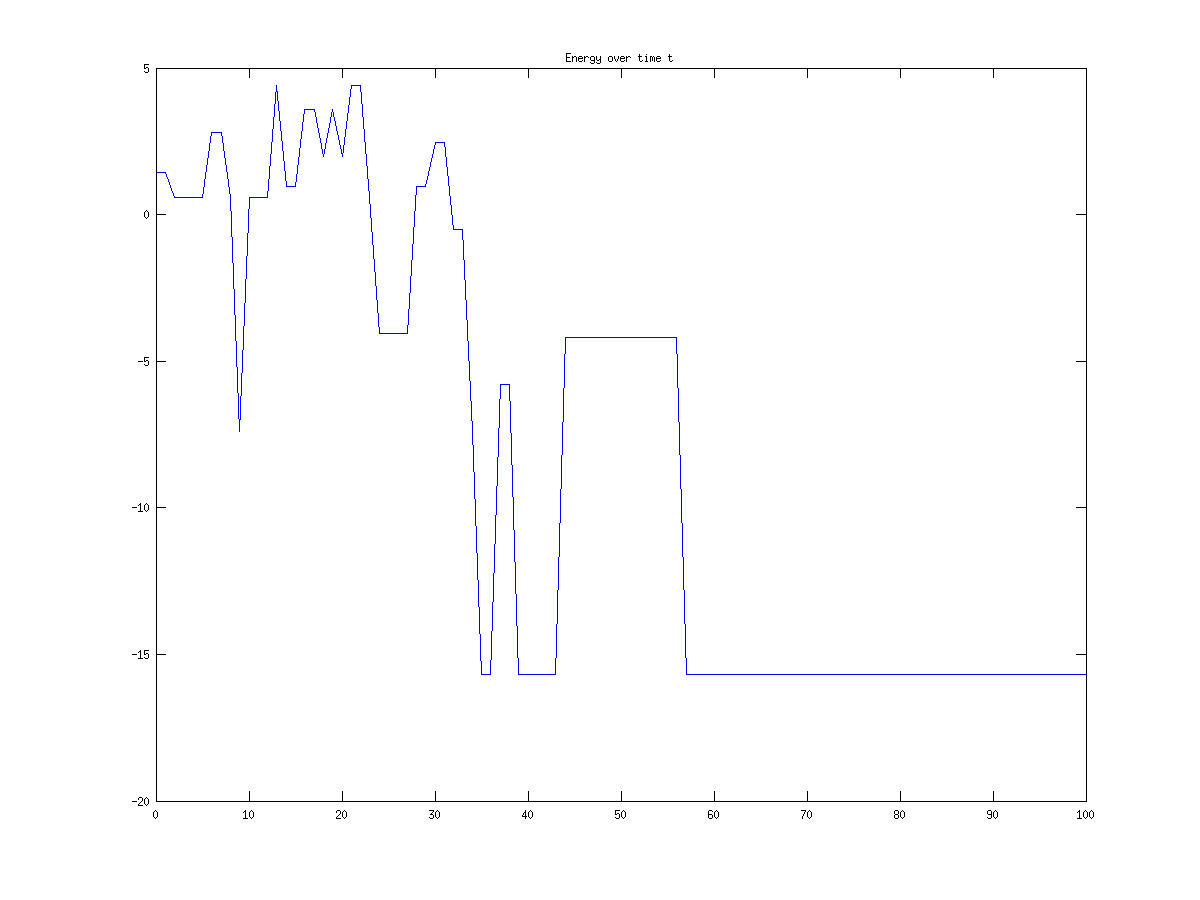
\includegraphics[width=10cm]{energy.png}
			\caption{Energy with respect to time}
		\end{figure}
		\begin{figure}[H]
			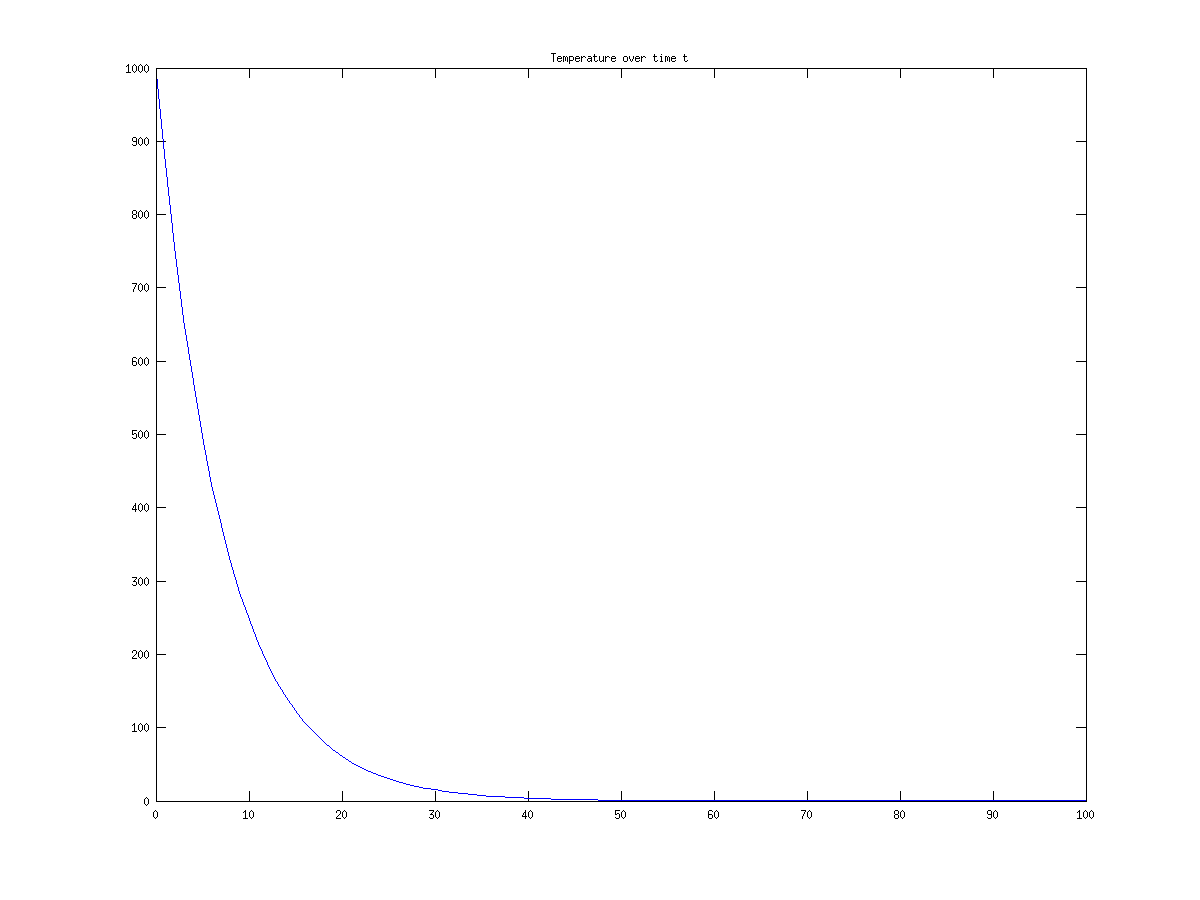
\includegraphics[width=10cm]{temperature.png}
			\caption{Temperature with respect to time}
		\end{figure}
		\begin{figure}[H]
			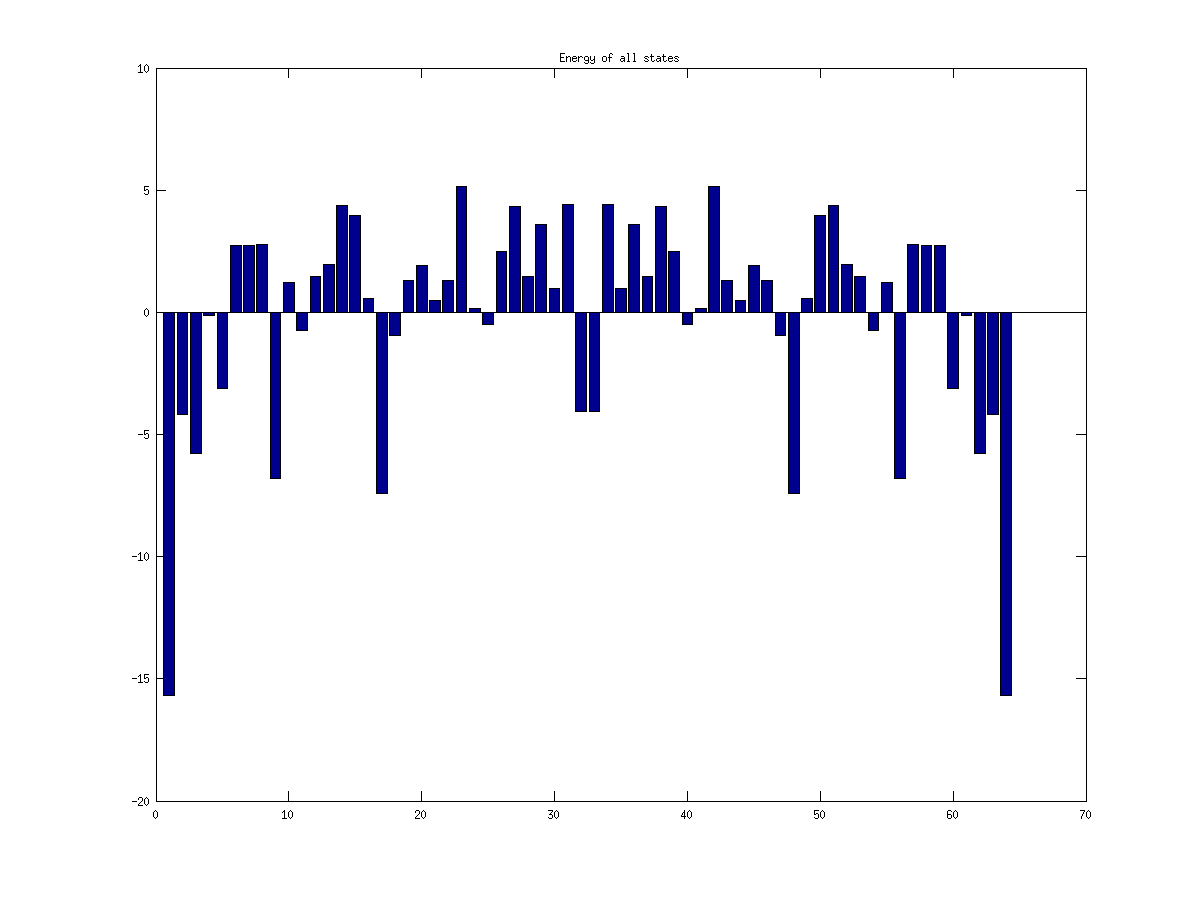
\includegraphics[width=10cm]{energies.png}
			\caption{Energies over all states}
		\end{figure}
		\begin{figure}[H]
			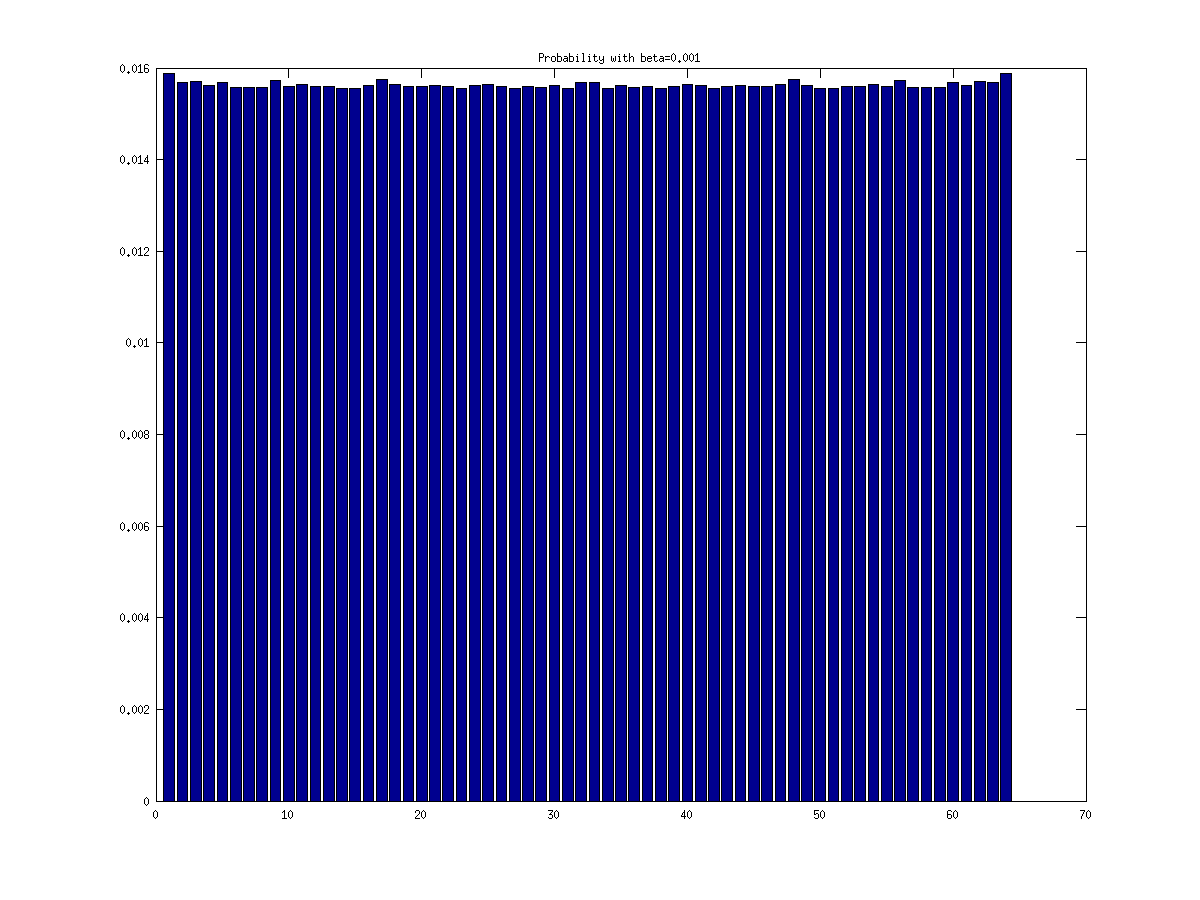
\includegraphics[width=10cm]{prob1.png}
			\caption{State probability with $\beta=0.001$}
		\end{figure}
		\begin{figure}[H]
			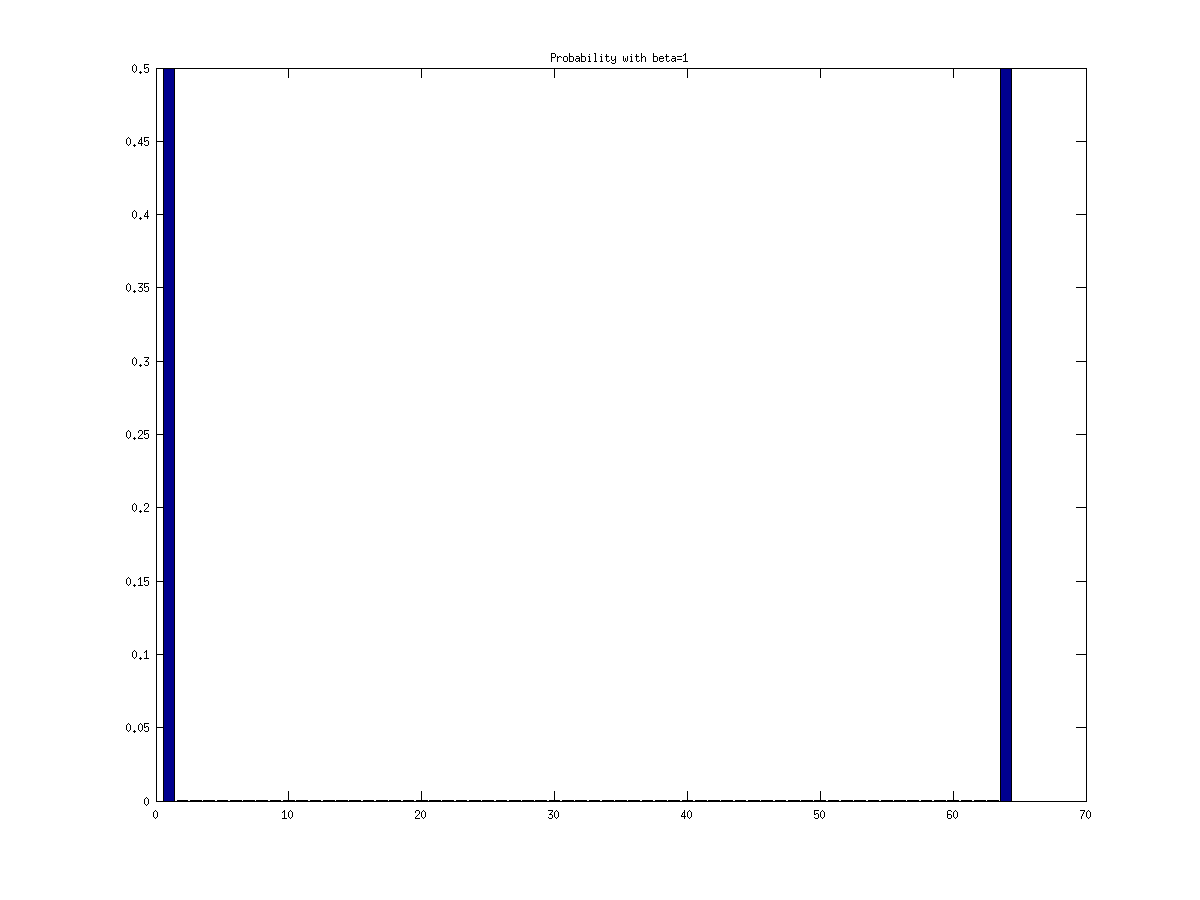
\includegraphics[width=10cm]{prob2.png}
			\caption{State probability with $\beta=1$}
		\end{figure}
	\subsection{Mean-Field Annealing}
		
		\begin{figure}[H]
			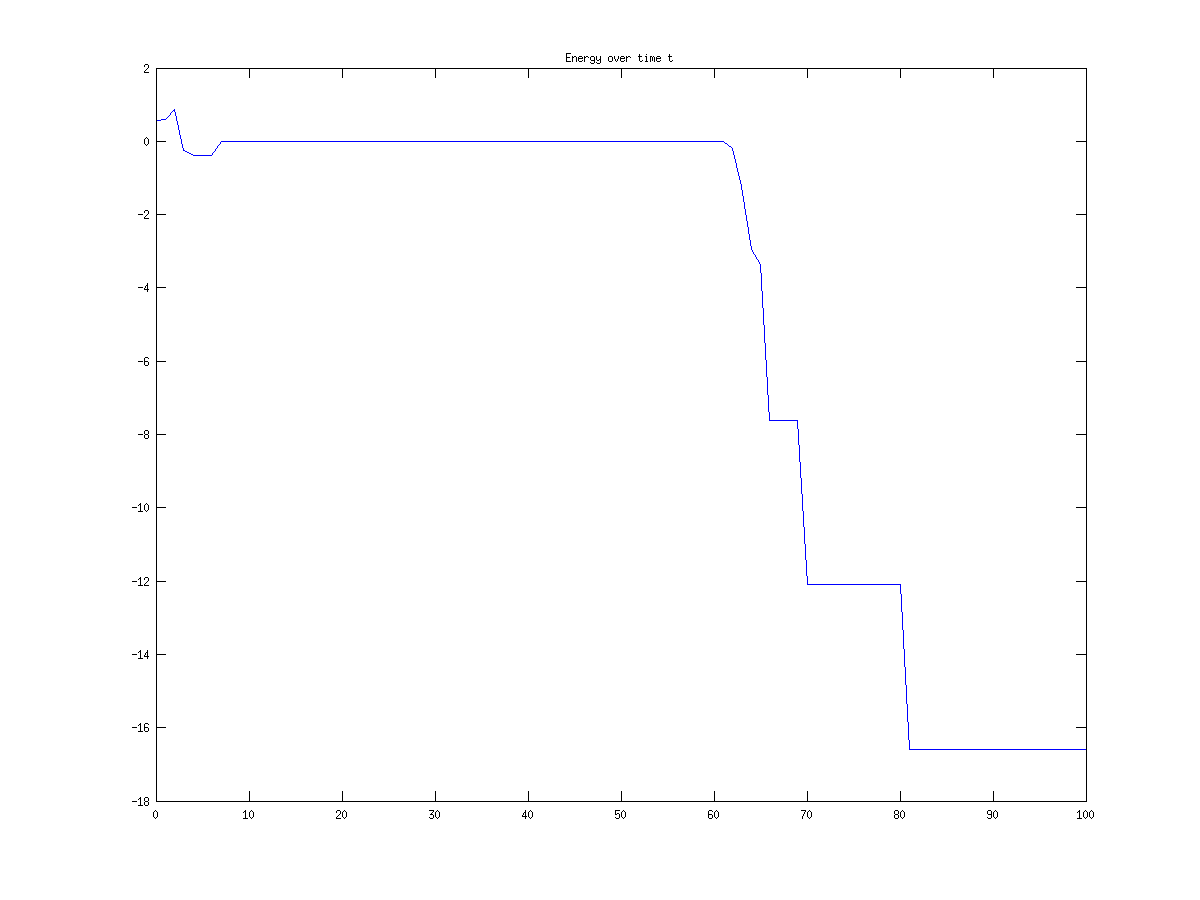
\includegraphics[width=10cm]{energy2.png}
			\caption{Energy with respect to time}		
		\end{figure}	
		
		\begin{figure}[H]
			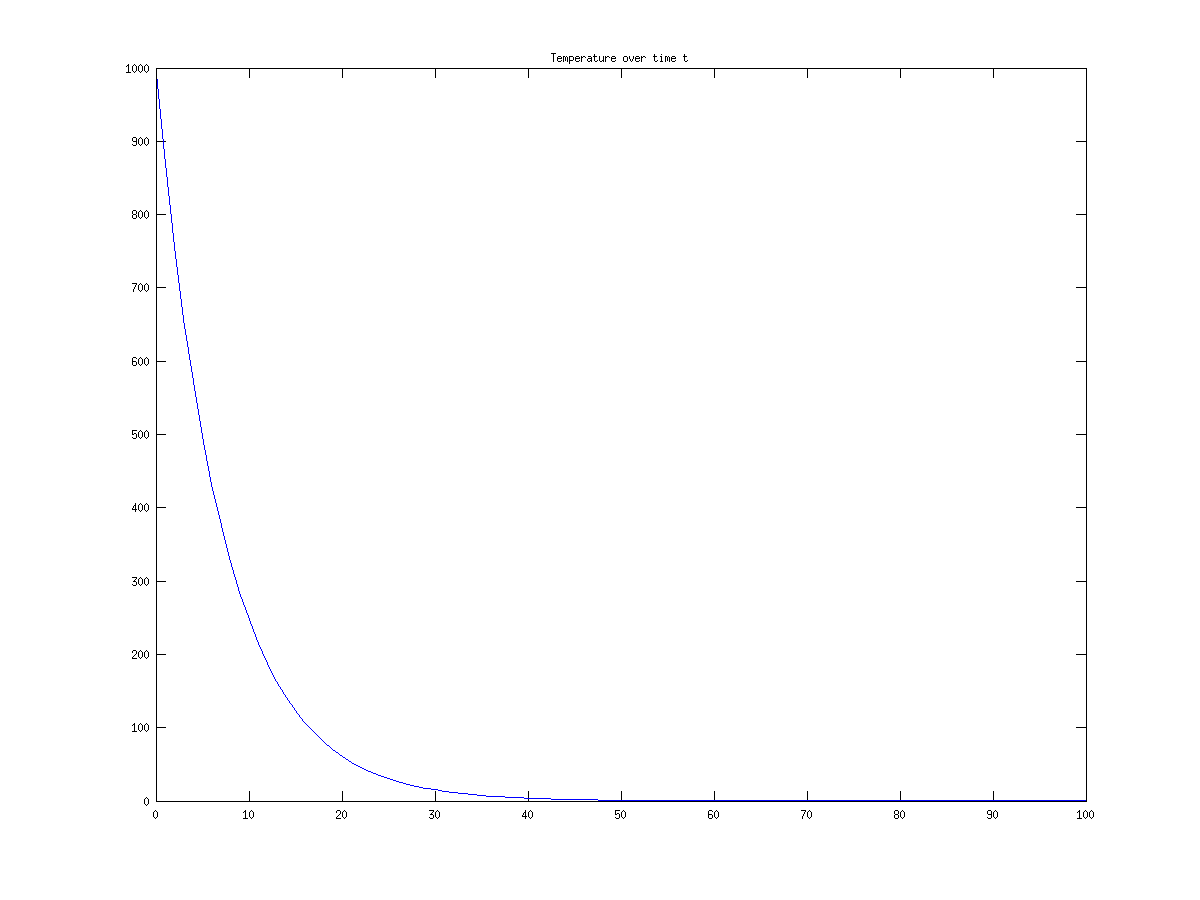
\includegraphics[width=10cm]{temperature2.png}
			\caption{Temperature with respect to time}
		\end{figure}
		
		One can see that the mean-field annealing converges slightly slower than the simulated annealing approach (after 80 iterations instead of 60 iterations). However, considering the fact that the state space of the mean-field annealing is vastly bigger, it is still a good result.
			
	
\end{document}
